\begin{center}
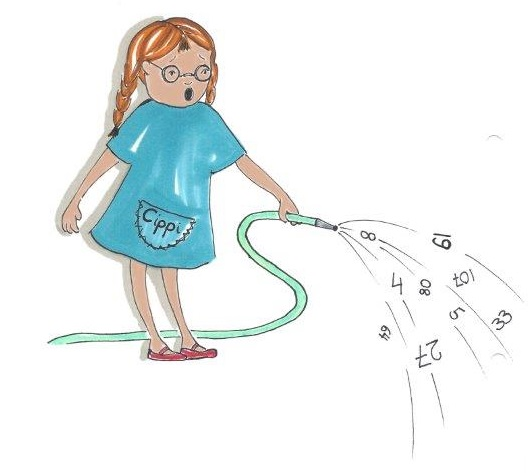
\includegraphics[width=0.6\textwidth]{content/3/chapter6/images/2.png}\\
Cippi waters the flowers
\end{center}

Coroutines are functions that can suspend and resume their execution while keeping their state. The evolution of functions in C++ goes one step further.

\begin{tcolorbox}[breakable,enhanced jigsaw,colback=red!5!white,colframe=red!75!black,title={The Challenge of Understanding Coroutines}]
	
It was quite a challenge for me to understand coroutines. I strongly suggest that you should not read the sections in the chapter in sequence. Skip in your first iteration the sections “The Framework”, and “The Workflow”. Furthermore, read the case studies “Variations of Futures”, “Modification and Generalization of a Generator”, and “Various Job Workflows”. Reading, studying, and playing with the provided examples should give you an initial intuition need for you to actually dive into details and the workflow of coroutines.
	
\end{tcolorbox}

What I present in this section as a new idea in C++20 is quite old. The term coroutine was coined by \href{https://en.wikipedia.org/wiki/Melvin_Conway}{Melvin Conway}. He used it in his publication on compiler construction in 1963. \href{https://en.wikipedia.org/wiki/Donald_Knuth}{Donald Knuth} called procedures a special case of coroutines. Sometimes, it just takes a while to get your ideas accepted.

\begin{center}
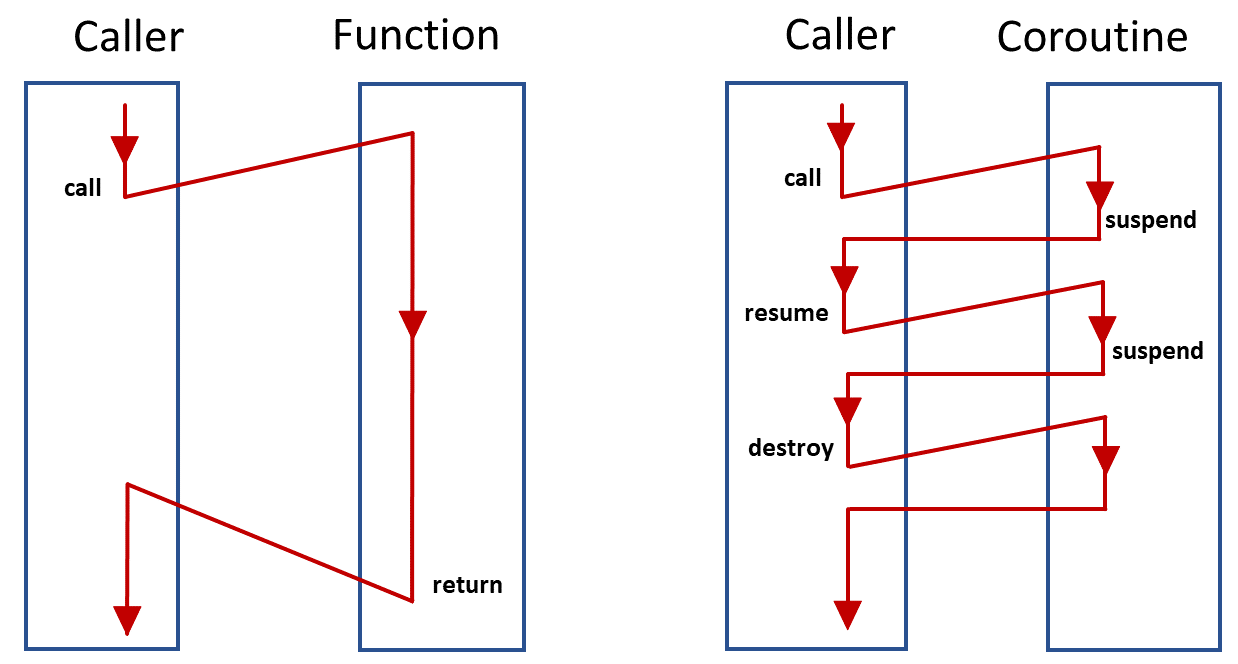
\includegraphics[width=0.6\textwidth]{content/3/chapter6/images/3.png}\\
Functions versus Coroutines
\end{center}

While you can only call a function and return from it, you can call a coroutine, suspend and resume it, and destroy a suspended coroutine.

With the new keywords co\_await and co\_yield, C++20 extends the execution of C++ functions with two new concepts.

Thanks to co\_await expression it is possible to suspend and resume the execution of the expression. If you use co\_await expression in a function func, the call auto getResult = func() does not block if the result of the function is not available. Instead of resource-consuming blocking, you have resource-friendly waiting.

co\_yield expression supports generator functions. The generator function returns a new value each time you call it. A generator function is a kind of data stream from which you can pick values. The data stream can be infinite. Therefore, we are at the center of lazy evaluation with C++.

\subsubsubsection{6.1.1\hspace{0.2cm} A Generator Function}

The following program is as simple as possible. The function getNumbers returns all integers from begin to end, incremented by inc. Value begin has to be smaller than end, and inc has to be positive.

\hspace*{\fill} \\ %插入空行
\noindent
A greedy generator function
\begin{lstlisting}[style=styleCXX]
// greedyGenerator.cpp

#include <iostream>
#include <vector>

std::vector<int> getNumbers(int begin, int end, int inc = 1) {

	std::vector<int> numbers;
	for (int i = begin; i < end; i += inc) {
		numbers.push_back(i);
	}
	
	return numbers;

}

int main() {

	std::cout << '\n';
	
	const auto numbers= getNumbers(-10, 11);
	
	for (auto n: numbers) std::cout << n << " ";
	
	std::cout << "\n\n";
	
	for (auto n: getNumbers(0, 101, 5)) std::cout << n << " ";
	
	std::cout << "\n\n";

}
\end{lstlisting}

Of course, I am reinventing the wheel with getNumbers, because that job could be done with \href{http://en.cppreference.com/w/cpp/algorithm/iota}{std::iota}.

For completeness, here is the output.

\begin{center}
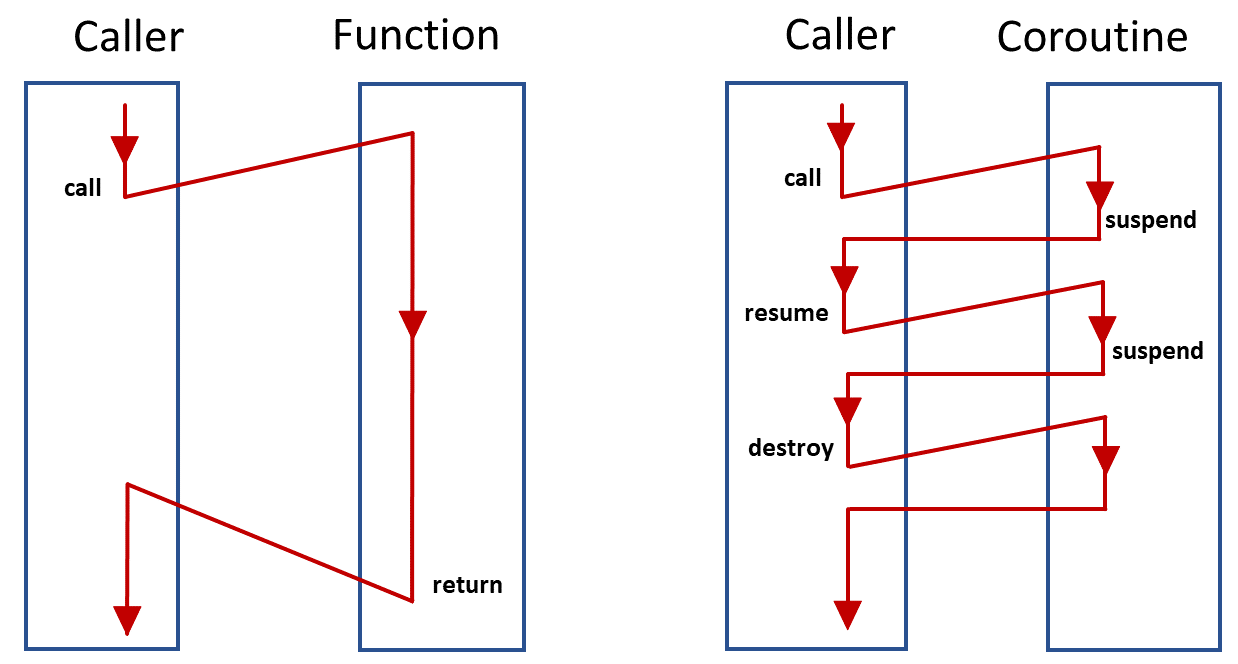
\includegraphics[width=0.4\textwidth]{content/3/chapter6/images/3.png}\\
A generator function
\end{center}

Two observations of the program greedyGenerator.cpp are essential. On the one hand, the vector numbers in line 8 always gets all values. This holds even if I’m only interested in the first 5 elements of a vector with 1000 elements. On the other hand, it’s quite easy to transform the function getNumbers into a lazy generator. The following program is intentionally not complete. The definition of the generator is still missing.

\hspace*{\fill} \\ %插入空行
\noindent
A lazy generator function
\begin{lstlisting}[style=styleCXX]
// lazyGenerator.cpp

#include <iostream>

generator<int> generatorForNumbers(int begin, int inc = 1) {

	for (int i = begin;; i += inc) {
		co_yield i;
	}

}

int main() {

	std::cout << '\n';
	
	const auto numbers = generatorForNumbers(-10);
	
	for (int i= 1; i <= 20; ++i) std::cout << numbers() << " ";
	
	std::cout << "\n\n";
	
	for (auto n: generatorForNumbers(0, 5)) std::cout << n << " ";
	
	std::cout << "\n\n";

}
\end{lstlisting}

While the function getNumbers in the file greedyGenerator.cpp returns a std::vector<int>, the coroutine generatorForNumbers in lazyGenerator.cpp returns a generator. The generator numbers in line 17 or generatorForNumbers(0, 5) in line 23 returns a new number on request. The range-based for loop triggers the query. Precisely, the query of the coroutine returns the value i via co\_yield i and immediately suspends its execution. If a new value is requested, the coroutine resumes its execution exactly at that place.

The expression generatorForNumbers(0, 5) in line 23 is a just-in-place use of a generator. I want to stress one point explicitly. The coroutine generatorForNumbers creates an infinite data stream because the for loop in line 8 has no end condition. This is fine if I only ask for a finite number of values, such as in line 20. This does not hold for line 23, since there is no end condition. Therefore, the expression runs forever.

\subsubsubsection{6.1.2\hspace{0.2cm} Characteristics}

Coroutines have a few unique characteristics.

\hspace*{\fill} \\ %插入空行
\noindent
\textbf{6.1.2.1\hspace{0.2cm} Typical Use Cases}

Coroutines are the usual way to write \href{https://en.wikipedia.org/wiki/Event-driven_programming}{event-driven applications}, which can be simulations, games, servers, user interfaces, or even algorithms. Coroutines are also typically used for \href{https://en.wikipedia.org/wiki/Computer_multitasking}{cooperative multitasking}. The key to cooperative multitasking is that each task takes as much time as it needs, but avoids sleeping or waiting, and instead allows some other task to run. Cooperative multitasking stands in contrast to pre-emptive multitasking, for which we have a scheduler that decides how long each task gets the CPU.

There are different kinds of coroutines.

\hspace*{\fill} \\ %插入空行
\noindent
\textbf{6.1.2.2\hspace{0.2cm} Underlying Concepts}

Coroutines in C++20 are asymmetric, first-class, and stackless.

The workflow of an asymmetric coroutine goes back to the caller. This does not hold for a symmetric coroutine. A symmetric coroutine can delegate its workflow to another coroutine.

First-class coroutines are similar to first-class functions, since coroutines behave like data. Behaving like data means that you can use them as arguments to or return values from functions, or store them in a variable.

A stackless coroutine can suspend and resume the top-level coroutine. The execution of the coroutine and the yielding from the coroutine comes back to the caller. The coroutine stores its state for resumption separate from the stack. Stackless coroutines are often called resumable functions.

\hspace*{\fill} \\ %插入空行
\noindent
\textbf{6.1.2.3\hspace{0.2cm} Design Goals}

Gor Nishanov describes in proposal \href{https://isocpp.org/files/papers/N4402.pdf}{N4402} the design goals of coroutines.

Coroutines should

\begin{itemize}
\item 
be highly scalable (to billions of concurrent coroutines)

\item 
have highly efficient resume and suspend operations comparable in cost to the overhead of a function

\item 
seamlessly interact with existing facilities with no overhead

\item 
have open-ended coroutine machinery allowing library designers to develop coroutine libraries exposing various high-level semantics such as generators, \href{https://tour.golang.org/concurrency/1}{goroutines}, tasks and more

\item 
usable in environments where exceptions are forbidden or not available
\end{itemize}

Due to the design goals of scalability and seamless interaction with existing facilities, the coroutines are stackless. In contrast, a stackful coroutine reserves a default stack of 1MB on Windows, and 2MB on Linux.

There are four ways for a function to become a coroutine.

\hspace*{\fill} \\ %插入空行
\noindent
\textbf{6.1.2.4\hspace{0.2cm} Becoming a Coroutine}

A function becomes a coroutine if it uses

\begin{itemize}
\item 
co\_return, or

\item 
co\_await, or

\item 
co\_yield, or a

\item 
co\_await expression in a range-based for loop.
\end{itemize}

\begin{tcolorbox}[breakable,enhanced jigsaw,colback=red!5!white,colframe=red!75!black,title={Distinguish Between the Coroutine Factory and the Coroutine Object}]
	
The term coroutine is often used for two different aspects of coroutines: the function invoking co\_return, co\_await, or co\_yield, and the coroutine object. Using one term for two different coroutine aspects may puzzle you (such as it did me). Let me clarify both terms.

\hspace*{\fill} \\ %插入空行
\noindent
A simple coroutine producing 2021
\begin{lstlisting}[style=styleCXX]
MyFuture<int> createFuture() {
	co_return 2021;
}

int main() {
	
	auto fut = createFuture();
	std::cout << "fut.get(): " << fut.get() << '\n';
	
}
\end{lstlisting}

This straightforward example has a function createFuture and returns an object of type MyFuture<int>. Both are called coroutines. To be specific, the function createFuture is a coroutine factory that returns a coroutine object. The coroutine object is a resumable object that implements the framework to model a specific behavior. I present in the section co\_return the implementation and the use of this straightforward coroutine.
	
\end{tcolorbox}

\hspace*{\fill} \\ %插入空行
\noindent
\textbf{6.1.2.4.1 \hspace{0.2cm} Restrictions}

Coroutines cannot have return statements or placeholder return types. This holds for unconstrained placeholders (auto), and constrained placeholders (concepts).

Additionally, functions having \href{https://en.cppreference.com/w/cpp/language/variadic_arguments}{variadic arguments}, constexpr functions, consteval functions, constructors, destructors, and the main function cannot be coroutines.

\subsubsubsection{6.1.3\hspace{0.2cm} The Framework}

The framework for implementing coroutines consists of more than 20 functions, some of which you must implement and some of which you may overwrite. Therefore, you can tailor the coroutine to your needs.

A coroutine is associated with three parts: the promise object, the coroutine handle, and the coroutine frame. The client gets the coroutine handle to interact with the promise object, which keeps its state in the coroutine frame.

\begin{center}
Promise object
\end{center}

\begin{table}[H]
\centering
\begin{tabular}{ll}
\textbf{Member Function}  & \textbf{Description}                                 \\ \hline
Default constructor       & A promise must be default constructible.             \\
initial\_suspend()        & Determines if the coroutine suspends before it runs. \\
final\_suspend noexcept() & Determines if the coroutine suspends before it ends. \\
unhandled\_exception()    & Called when an exception happens.                    \\
get\_return\_object()     & Returns the coroutine object (resumable object).     \\
return\_value(val)        & Is invoked by co\_return val.                        \\
return\_void()            & Is invoked by co\_return.                            \\
yield\_value(val)         & Is invoked by co\_yield val.                        
\end{tabular}
\end{table}

The compiler automatically invokes these functions during its execution of the coroutine. The section workflow presents this workflow in detail.

The function get\_return\_object returns a resumable object that the client uses to interact with the coroutine. A promise needs at least one of the member functions return\_value, return\_void, or yield\_value. You don’t need to define the member functions return\_value or return\_void if your coroutine never ends.

The three functions yield\_value, initial\_suspend, and final\_suspend return awaitables. An Awaitable is something that you can await on. The awaitable determines if the coroutine pauses or not.

\hspace*{\fill} \\ %插入空行
\noindent
\textbf{6.1.3.2\hspace{0.2cm} Coroutine Handle}

The coroutine handle is a non-owning handle to resume or destroy the coroutine frame from the outside. The coroutine handle is part of the resumable function.

The following code snippet shows a simple Generator having a coroutine handle coro.

\hspace*{\fill} \\ %插入空行
\noindent
A coroutine handle
\begin{lstlisting}[style=styleCXX]
template<typename T>
struct Generator {

	struct promise_type;
	using handle_type = std::coroutine_handle<promise_type>;
	
	Generator(handle_type h): coro(h) {}
	handle_type coro;
	
	~Generator() {
		if ( coro ) coro.destroy();
	}
	T getValue() {
		return coro.promise().current_value;
	}
	bool next() {
		coro.resume();
		return not coro.done();
	}
	...
}
\end{lstlisting}

The constructor (line 7) gets the coroutine handle to the promise that has type \href{https://en.cppreference.com/w/cpp/coroutine/coroutine_handle}{std::coroutine\_handle<promise\_type>}. The member functions next (line 16) and getValue (line 13) allow a client to resume the promise (gen.next()) or ask for its value (gen.getValue()) using the coroutine handle.

\hspace*{\fill} \\ %插入空行
\noindent
Invoking a coroutine
\begin{lstlisting}[style=styleCXX]
Generator<int> coroutineFactory(); // function that returns a coroutine object

auto gen = coroutineFactory();
gen.next();
auto result = gen.getValue();
\end{lstlisting}

Internally, both functions trigger the coroutine handle coro (line 8) to

\begin{itemize}
\item 
resume the coroutine: coro.resume() (line 17) or coro();

\item 
destroy the coroutine: coro.destroy() (line 11);

\item 
check the state of the coroutine: coro (line 11).
\end{itemize}

The coroutine is automatically destroyed when its function body ends. The call coro only returns true at its final suspension point.

\begin{tcolorbox}[breakable,enhanced jigsaw,colback=red!5!white,colframe=red!75!black,title={The resumable object requires an inner type promise\_type}]
A resumable object such as Generator must have an inner type promise\_type. Alternatively, you can specialize \href{https://en.cppreference.com/w/cpp/coroutine/coroutine_traits}{std::coroutine\_traits} on Generator and define a public member promise\_type in it: std::coroutine\_traits<Generator>.
\end{tcolorbox}

\hspace*{\fill} \\ %插入空行
\noindent
\textbf{6.1.3.3\hspace{0.2cm} Coroutine Frame}

The coroutine frame is an internal, typically heap-allocated state. It consists of the already mentioned promise object, the coroutine’s copied parameters, the representation of the suspension points, local variables whose lifetime ends before the current suspension point, and local variables whose lifetime exceed the current suspension point.

Two requirements are necessary to optimize out the allocation of the coroutine:

\begin{enumerate}
\item 
The lifetime of the coroutine has to be nested inside the lifetime of the caller

\item 
The caller of the coroutine knows the size of the coroutine frame.

\end{enumerate}

\subsubsubsection{6.1.4\hspace{0.2cm} Awaitables and Awaiters}

The three functions of a promise object prom yield\_value, initial\_suspend, and final\_suspend return awaitables.

\hspace*{\fill} \\ %插入空行
\noindent
\textbf{6.1.4.1\hspace{0.2cm} Awaitables}

An Awaitable is something you can await on. The awaitable determines if the coroutine pauses or not.

Essentially, the compiler generated the three function calls using the promise prom and the co\_await operator.

\begin{center}
Compiler-generated function calls
\end{center}

\begin{table}[H]
\centering
\begin{tabular}{ll}
\textbf{Call}           & \textbf{Compiler generated call}   \\ \hline
yield value             & co\_await prom.yield\_value(value) \\
prom.initial\_suspend() & co\_await prom.initial\_suspend()  \\
prom.final\_suspend()   & co\_await prom.final\_suspend()   
\end{tabular}
\end{table}

The co\_await operator needs an awaitable as argument. Awaitables have to implement the concept Awaitable.

\hspace*{\fill} \\ %插入空行
\noindent
\textbf{6.1.4.2\hspace{0.2cm} The Concept Awaitable}

The concept Awaitable requires three functions.

\begin{center}
The concept Awaitable
\end{center}

\begin{table}[H]
\centering
\begin{tabular}{ll}
\textbf{Function} & \textbf{Description}                                  \\ \hline
await\_ready & \begin{tabular}[c]{@{}l@{}}Indicates if the result is ready. When it returns false,\\ await\_suspend is called.\end{tabular} \\
await\_suspend    & Schedule the coroutine for resumption or destruction. \\
await\_resume     & Provides the result for the co\_await exp expression.
\end{tabular}
\end{table}

The C++20 standard already defines two basic awaitables: std::suspend\_always, and std::suspend\_never.

\hspace*{\fill} \\ %插入空行
\noindent
\textbf{6.1.4.3\hspace{0.2cm} std::suspend\_always and std::suspend\_never}

As its name suggests, the Awaitable suspend\_always always suspends. Therefore, the call await\_ready returns false.

\hspace*{\fill} \\ %插入空行
\noindent
The Awaitable std::suspend\_always
\begin{lstlisting}[style=styleCXX]
struct suspend_always {
	constexpr bool await_ready() const noexcept { return false; }
	constexpr void await_suspend(std::coroutine_handle<>) const noexcept {}
	constexpr void await_resume() const noexcept {}
};
\end{lstlisting}

The opposite holds for suspend\_never. It never suspends and, hence, the call await\_ready returns
true.

\hspace*{\fill} \\ %插入空行
\noindent
The Awaitable std::suspend\_never
\begin{lstlisting}[style=styleCXX]
struct suspend_never {
	constexpr bool await_ready() const noexcept { return true; }
	constexpr void await_suspend(std::coroutine_handle<>) const noexcept {}
	constexpr void await_resume() const noexcept {}
};
\end{lstlisting}

The awaitables std::suspend\_always and std::suspend\_never are the basic building blocks for functions, such as initial\_suspend and final\_suspend. Both functions are automatically executed when the coroutine is exected: initial\_suspend at the beginning and final\_suspend at the end end of the coroutine.

\hspace*{\fill} \\ %插入空行
\noindent
\textbf{6.1.4.4\hspace{0.2cm} initial\_suspend}

When the member function initial\_suspend returns std::suspend\_always, the coroutine suspends at its beginning. When returning std::suspend\_never, the coroutine does not pause.

\begin{itemize}
\item 
A lazy coroutine that pauses immediately

\hspace*{\fill} \\ %插入空行
\noindent
A lazy coroutine
\begin{lstlisting}[style=styleCXX]
std::suspend_always initial_suspend() {
	return {};
}
\end{lstlisting}

\item 
An eager coroutine that runs immediately

\hspace*{\fill} \\ %插入空行
\noindent
A eager coroutine
\begin{lstlisting}[style=styleCXX]
std::suspend_never initial_suspend() {
	return {};
}
\end{lstlisting}
\end{itemize}


\hspace*{\fill} \\ %插入空行
\noindent
\textbf{6.1.4.5\hspace{0.2cm} final\_suspend}

When the member function final\_suspend returns std::suspend\_always, the coroutine suspends at its end. When returning std::suspend\_never, the coroutine does not pause.

\begin{itemize}
\item 
A lazy coroutine that pauses at its end

\hspace*{\fill} \\ %插入空行
\noindent
A lazy coroutine that finally pauses
\begin{lstlisting}[style=styleCXX]
std::suspend_always final_suspend noexcept noexcept noexcept noexcept() {
	return {};
}
\end{lstlisting}

\item 
An eager coroutine that doesn’t pause at its end

\hspace*{\fill} \\ %插入空行
\noindent
A eager coroutine that doesn’t pause
\begin{lstlisting}[style=styleCXX]
std::suspend_never final_suspend() noexcept {
	return {};
}
\end{lstlisting}
\end{itemize}

So far, we have only Awaitables, but we need something to await for. Let me fill the gap and write about Awaiters.

\hspace*{\fill} \\ %插入空行
\noindent
\textbf{6.1.4.6\hspace{0.2cm} Awaiter}

There are essentially two ways to get an Awaiter.

\begin{itemize}
\item 
A co\_await operator is defined.

\item 
The Awaitable becomes the Awaiter.
\end{itemize}

Remember, when co\_await expression is invoked, the expression is an Awaitable. Further, an expression is a call on the promise object (Awaitable): prom.yield\_value(value), prom.initial\_suspend(), or prom.final\_suspend(). For readability, I rename in the following lines promise object prom to awaitable.

Now, the compiler performs the following lookup rule to get an Awaiter:

\begin{enumerate}
\item 
It looks for the co\_await operator on the promise object and returns an Awaiter:
\begin{lstlisting}[style=styleCXX]
awaiter = awaitable.operator co_await();
\end{lstlisting}

\item 
It looks for a freestanding co\_wait operator and returns an Awaiter:
\begin{lstlisting}[style=styleCXX]
awaiter = operator co_await();
\end{lstlisting}

\item 
If there is no co\_wait operator defined, the Awaitable becomes the Awaiter:
\begin{lstlisting}[style=styleCXX]
awaiter = awaitable;
\end{lstlisting}
\end{enumerate}

\begin{tcolorbox}[breakable,enhanced jigsaw,colback=blue!5!white,colframe=blue!75!black,title={awaiter = awaitable}]
When you study my coroutine implementations in this chapter, you may notice that I use most of the time that an Awaitable implicitly becomes an Awaiter. Only the example to thread synchronization uses the co\_await operator to get the Awaiter.
\end{tcolorbox}

After these static aspects of coroutines, I want to continue with their dynamic aspects.

\subsubsubsection{6.1.5\hspace{0.2cm} The Workflows}

The compiler transforms your coroutine and runs two workflows: the outer promise workflow and the inner awaiter workflow.

\hspace*{\fill} \\ %插入空行
\noindent
\textbf{6.1.5.1\hspace{0.2cm} The Promise Workflow}

When you use co\_yield, co\_await, or co\_return in a function, the function becomes a coroutine, and the compiler transforms its body to something equivalent to the following lines.

\hspace*{\fill} \\ %插入空行
\noindent
The transformed coroutine
\begin{lstlisting}[style=styleCXX]
{
	Promise prom;
	co_await prom.initial_suspend();
	try {
		<function body having co_return, co_yield, or co_wait>
	}
	catch (...) {
		prom.unhandled_exception();
	}
FinalSuspend:
	co_await prom.final_suspend();
}
\end{lstlisting}

The compiler automatically runs the transformed code using the functions of the promise object. In short, I call this workflow the promise workflow. Here are the main steps of this workflow.

\begin{itemize}
\item 
Coroutine begins execution
\begin{itemize}
\item 
allocates the coroutine frame if necessary

\item 
copies all function parameters to the coroutine frame

\item 
creates the prom object prom (line 2)

\item 
calls prom.get\_return\_object() to create the coroutine handle, and keeps it in a local variable. The result of the call will be returned to the caller when the coroutine first suspends.

\item 
calls prom.initial\_suspend() and co\_awaits its result. The promise type typically returns suspend\_never for eagerly-started coroutines or suspend\_always for lazily-started coroutines. (line 3)

\item 
the body of the coroutine is executed when co\_await prom.initial\_suspend() resumes
\end{itemize}

\item 
Coroutine reaches a suspension point
\begin{itemize}
\item 
the return object (prom.get\_return\_object()) is returned to the caller which resumed the coroutine
\end{itemize}

\item 
Coroutine reaches co\_return
\begin{itemize}
\item 
calls prom.return\_void() for co\_return or co\_return expression, where expression has type void

\item 
calls prom.return\_value(expression) for co\_return expression, where expression has non-void type.

\item 
destroys all stack-created variables

\item 
calls prom.final\_suspend() and co\_awaits its result
\end{itemize}

\item 
Coroutine is destroyed (by terminating via co\_return an uncaught exception, or via the coroutine handle)
\begin{itemize}
\item 
calls the destruction of the promise object

\item 
calls the destructor of the function parameters

\item 
frees the memory used by the coroutine frame

\item 
transfers control back to the caller
\end{itemize}
\end{itemize}

When a coroutine ends with an uncaught exception, the following happens:

\begin{itemize}
\item 
catches the exception and calls prom.unhandled\_exception() from the catch block

\item 
calls prom.final\_suspend() and co\_awaits the result (line 11)
\end{itemize}

When you use co\_await expr in a coroutine, or the compiler implicitly invokes co\_await prom.initial\_suspend(), co\_await prom.final.suspend(), or co\_await prom.yield\_value(value), a second, inner awaitable workflow starts.

\hspace*{\fill} \\ %插入空行
\noindent
\textbf{6.1.5.2\hspace{0.2cm} The Awaiter Workflow}

Using co\_await expr causes the compiler to transform the code based on the functions await\_ready, await\_suspend, and await\_resume. Consequently, I call the execution of the transformed code the awaiter workflow.

The compiler generates approximately the following code using the awaitable. For simplicity, I ignore exception handling and describe the workflow with comments.

\hspace*{\fill} \\ %插入空行
\noindent
The generated Awaiter Workflow
\begin{lstlisting}[style=styleCXX]
awaitable.await_ready() returns false:

	suspend coroutine
	
	awaitable.await_suspend(coroutineHandle) returns:
		void:
			awaitable.await_suspend(coroutineHandle);
			coroutine keeps suspended
			return to caller
	
	bool:
		bool result = awaitable.await_suspend(coroutineHandle);
		if result:
			coroutine keep suspended
			return to caller
		else:
			go to resumptionPoint
	
	another coroutine handle:
		auto anotherCoroutineHandle = awaitable.await_suspend(coroutineHandle);
		anotherCoroutineHandle.resume();
		return to caller

resumptionPoint:

return awaitable.await_resume();
\end{lstlisting}

The workflow is only executed if awaitable.await\_ready() returns false (line 1). In case it returns true, the coroutine is ready and returns with the result of the call awaitable.await\_resume() (line 27).

Let me assume that awaitable.await\_ready() returns false. First, the coroutine is suspended (line 3), and immediately the return value of awaitable.await\_suspend() is evaluated. The return type can be void (line 7), a boolean (line 12), or another coroutine handle (line 20), such as anotherCoroutineHandle. Depending on the return type, the program flow returns or another coroutine is executed.

\begin{center}
Return value of awaitable.await\_suspend()
\end{center}

\begin{table}[H]
\centering
\begin{tabular}{ll}
\textbf{Type}          & \textbf{Description}                                      \\ \hline
void                   & The coroutine keeps suspended and returns to the caller.  \\
bool &
\begin{tabular}[c]{@{}l@{}}bool == true: The coroutine keeps suspended and returns to the caller.\\ bool == false: The coroutine is resumed and does not return to the caller.\end{tabular} \\
anotherCoroutineHandle & The other coroutine is resumed and returns to the caller.
\end{tabular}
\end{table}


Whats happens in case an exception is thrown? It makes a difference if the exception occurs in await\_read, await\_suspend, or await\_resume.

\begin{itemize}
\item 
await\_ready: The coroutine is not suspended, nor are the calls await\_suspend or await\_resume evaluated.

\item 
await\_suspend: The exception is caught, the coroutine is resumed, and the exception rethrown.
await\_resume is not called.

\item 
await\_resume: await\_ready and await\_suspend are evaluated and all values are returned. Of course, the call await\_resume does not return a result.
\end{itemize}

Let me put theory into practice.

\subsubsubsection{6.1.6\hspace{0.2cm} co\_return}

A coroutine uses co\_return as its return statement.

\hspace*{\fill} \\ %插入空行
\noindent
\textbf{6.1.6.1\hspace{0.2cm} A Future}

Admittedly, the coroutine in the following program eagerFuture.cpp is the simplest coroutine I can imagine that still does something meaningful: it automatically stores the result of its invocation.

\hspace*{\fill} \\ %插入空行
\noindent
An eager future
\begin{lstlisting}[style=styleCXX]
// eagerFuture.cpp

#include <coroutine>
#include <iostream>
#include <memory>

template<typename T>
struct MyFuture {
	std::shared_ptr<T> value;
	MyFuture(std::shared_ptr<T> p): value(p) {}
	~MyFuture() { }
		T get() {
		return *value;
	}

	struct promise_type {
		std::shared_ptr<T> ptr = std::make_shared<T>();
		~promise_type() { }
		MyFuture<T> get_return_object() {
			return ptr;
		}
		void return_value(T v) {
			*ptr = v;
		}
		std::suspend_never initial_suspend() {
			return {};
		}
		std::suspend_never final_suspend() noexcept {
			return {};
		}
		void unhandled_exception() {
			std::exit(1);
		}
	};
};

MyFuture<int> createFuture() {
	co_return 2021;
}

int main() {

	std::cout << '\n';
	
	auto fut = createFuture();
	std::cout << "fut.get(): " << fut.get() << '\n';
	
	std::cout << '\n';

}
\end{lstlisting}

MyFuture behaves as a \href{https://en.cppreference.com/w/cpp/thread/future}{future}, which runs immediately. The call of the coroutine createFuture (line 45) returns the future, and the call fut.get (line 46) picks up the result of the associated promise.

There is one subtle difference to a future, the return value of the coroutine createFuture is available after its invocation. Due to the lifetime issues, the return value is managed by a std::shared\_ptr (lines 9 and 17). The coroutine always uses std::suspend\_never (lines 25, and 28) and, therefore, neither suspends before it runs nor after. This means the coroutine is executed when the function createFuture is invoked. The member function get\_return\_object (line 19) creates and stores the handle to the coroutine object, and return\_value (lines 22) stores the result of the coroutine, which was provided by co\_return 2021 (line 38). The client invokes fut.get (line 46) and uses the future as a handle to the promise. The member function get returns the result to the client (line 13).

\begin{tcblisting}{breakable,commandshell={}}
fut.get(): 2021
\end{tcblisting}

\begin{center}
An eager future
\end{center}

You may think that it is not worth the effort of implementing a coroutine that behaves just like a function. You are right! However, this simple coroutine is an ideal starting point for writing various implementations of futures. Read more about Variations of Futures in chapter case studies.

\subsubsubsection{6.1.7\hspace{0.2cm} co\_yield}

Thanks to co\_yield you can implement a generator generating an infinite data stream from which you can successively query values. The return type of the generator generatorForNumbers(int begin, int inc= 1) is generator<int>, where generator internally holds a special promise p such that a call co\_yield i is equivalent to a call co\_await p.yield\_value(i). Statement co\_yield i can be called an arbitrary number of times. Immediately after each call, the execution of the coroutine is suspended.

\hspace*{\fill} \\ %插入空行
\noindent
\textbf{6.1.7.1\hspace{0.2cm} An Infinite Data Stream}

The program infiniteDataStream.cpp produces an infinite data stream. The coroutine getNext uses co\_yield to create a data stream that starts at start and gives on request the next value, incremented by step.

\hspace*{\fill} \\ %插入空行
\noindent
An infinite data stream
\begin{lstlisting}[style=styleCXX]
// infiniteDataStream.cpp

#include <coroutine>
#include <memory>
#include <iostream>

template<typename T>
struct Generator {

	struct promise_type;
	using handle_type = std::coroutine_handle<promise_type>;
	
	Generator(handle_type h): coro(h) {} // (3)
	handle_type coro;
	
	~Generator() {
		if ( coro ) coro.destroy();
	}

	Generator(const Generator&) = delete;
	Generator& operator = (const Generator&) = delete;
	Generator(Generator&& oth) noexcept : coro(oth.coro) {
		oth.coro = nullptr;
	}
		Generator& operator = (Generator&& oth) noexcept {
		coro = oth.coro;
		oth.coro = nullptr;
		return *this;
	}
	T getValue() {
		return coro.promise().current_value;
	}
	bool next() { // (5)
		coro.resume();
		return not coro.done();
	}
	struct promise_type {
		promise_type() = default; // (1)
		
		~promise_type() = default;
		
		auto initial_suspend() { // (4)
			return std::suspend_always{};
		}
		auto final_suspend() noexcept {
			return std::suspend_always{};
		}
		auto get_return_object() { // (2)
			return Generator{handle_type::from_promise(*this)};
		}
		auto return_void() {
			return std::suspend_never{};
		}
	
		auto yield_value(const T value) { // (6)
			current_value = value;
			return std::suspend_always{};
		}
		void unhandled_exception() {
			std::exit(1);
		}
		T current_value;
	};

};

Generator<int> getNext(int start = 0, int step = 1) {
	auto value = start;
	while (true) {
		co_yield value;
		value += step;
	}
}

int main() {

	std::cout << '\n';
	
	std::cout << "getNext():";
	auto gen = getNext();
	for (int i = 0; i <= 10; ++i) {
		gen.next();
		std::cout << " " << gen.getValue(); // (7)
	}
	
	std::cout << "\n\n";
	
	std::cout << "getNext(100, -10):";
	auto gen2 = getNext(100, -10);
	for (int i = 0; i <= 20; ++i) {
		gen2.next();
		std::cout << " " << gen2.getValue();
	}
	
	std::cout << '\n';

}
\end{lstlisting}

The main program creates two coroutines. The first one gen (line 79) returns the values from 0 to 10, and the second one gen2 (line 88) the values from 100 to -100. Before I dive into the workflow, thanks to the online compiler \href{https://wandbox.org/}{Wandbox}, here is the output of the program.

\begin{center}
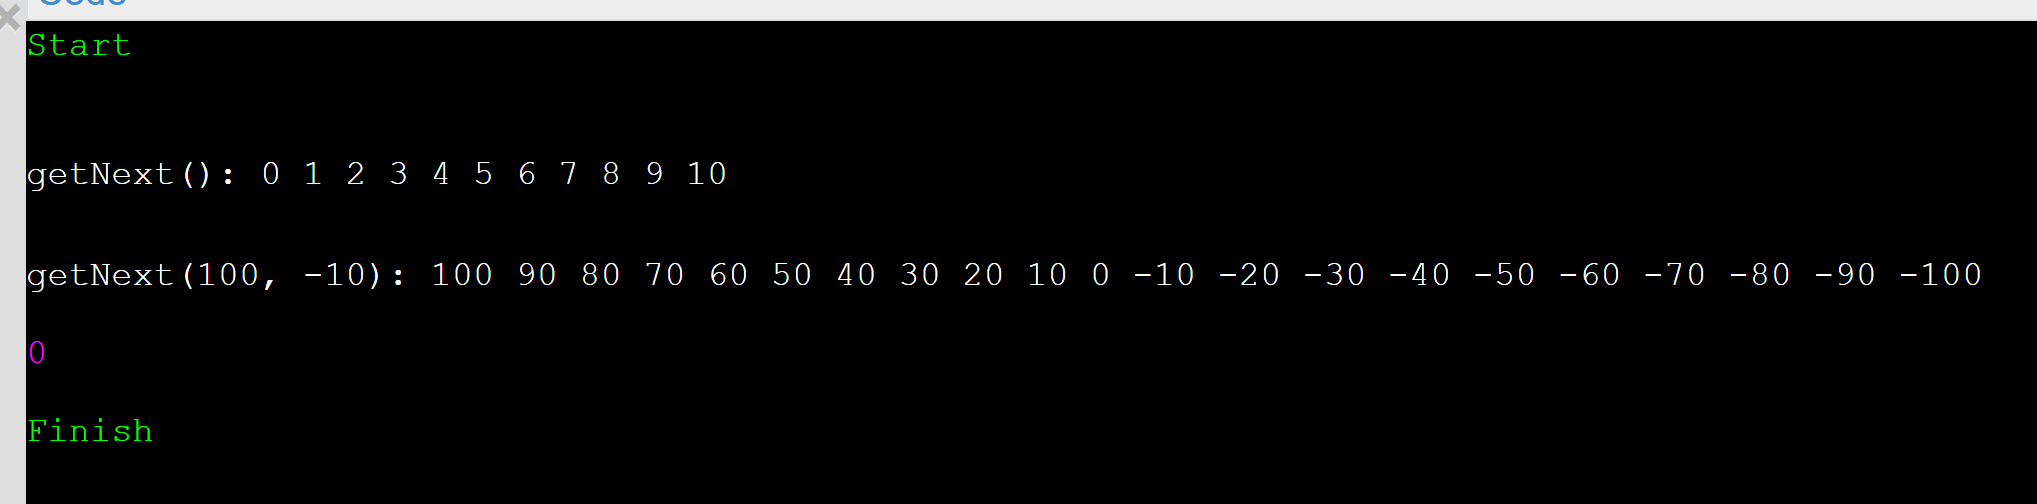
\includegraphics[width=0.4\textwidth]{content/3/chapter6/images/5.png}\\
An infinite data stream
\end{center}

The numbers in the program infiniteDataStream.cpp stand for the steps in the first iteration of the workflow.

\begin{enumerate}
\item 
creates the promise

\item 
calls promise.get\_return\_object() and keeps the result in a local variable

\item 
creates the generator

\item 
calls promise.initial\_suspend(). The generator is lazy and, therefore, always suspends.

\item 
asks for the next value and returns if the generator is consumed

\item 
triggered by the co\_yield call. The next value is available thereafter.

\item 
gets the next value
\end{enumerate}

In additional iterations, only steps 5, 6, and 7 are performed.

Section Modification and Generalization of Threads in chapter case studies discusses further improvements and modifications of the generator infiniteDataStream.cpp

\subsubsubsection{6.1.8\hspace{0.2cm} co\_await}

co\_await eventually causes the execution of the coroutine to be suspended or resumed. The expression exp in co\_await exp has to be a so-called awaitable expression, i.e. which must implement a specific interface, consisting of the three functions await\_ready, await\_suspend, and await\_resume.

A typical use case for co\_await is a server that waits for events.

\hspace*{\fill} \\ %插入空行
\noindent
A blocking server
\begin{lstlisting}[style=styleCXX]
Acceptor acceptor{443};
while (true) {
	Socket socket = acceptor.accept(); // blocking
	auto request = socket.read(); // blocking
	auto response = handleRequest(request);
	socket.write(response); // blocking
}
\end{lstlisting}

The server is quite simple because it sequentially answers each request in the same thread. The server listens on port 443 (line 1), accepts the connection (line 3), reads the incoming data from the client (line 4), and writes its answer to the client (line 6). The calls in lines 3, 4, and 6 are blocking.

Thanks to co\_await, the blocking calls can now be suspended and resumed.

\hspace*{\fill} \\ %插入空行
\noindent
A waiting server
\begin{lstlisting}[style=styleCXX]
Acceptor acceptor{443};
while (true) {
	Socket socket = co_await acceptor.accept();
	auto request = co_await socket.read();
	auto response = handleRequest(request);
	co_await socket.write(response);
}
\end{lstlisting}

Before I present the challenging example of thread synchronization with coroutines, I want to start with something straightforward: starting a job on request.

\hspace*{\fill} \\ %插入空行
\noindent
\textbf{6.1.8.1\hspace{0.2cm} Starting a Job on Request}

The coroutine in the following example is as simple as it can be. It awaits on the predefined Awaitable std::suspend\_never().

\hspace*{\fill} \\ %插入空行
\noindent
Starting a job on request
\begin{lstlisting}[style=styleCXX]
// startJob.cpp

#include <coroutine>
#include <iostream>

struct Job {
	struct promise_type;
	using handle_type = std::coroutine_handle<promise_type>;
	handle_type coro;
	Job(handle_type h): coro(h){}
	~Job() {
		if ( coro ) coro.destroy();
	}
	void start() {
		coro.resume();
	}


	struct promise_type {
		auto get_return_object() {
			return Job{handle_type::from_promise(*this)};
		}
		std::suspend_always initial_suspend() {
			std::cout << " Preparing job" << '\n';
			return {};
		}
		std::suspend_always final_suspend() noexcept {
			std::cout << " Performing job" << '\n';
			return {};
		}
		void return_void() {}
		void unhandled_exception() {}
	
	};
};

Job prepareJob() {
	co_await std::suspend_never();
}

int main() {

	std::cout << "Before job" << '\n';
	
	auto job = prepareJob();
	job.start();
	
	std::cout << "After job" << '\n';

}
\end{lstlisting}

You may think that the coroutine prepareJob (line 37) is meaningless because the Awaitable always suspends. No! The function prepareJob is at least a coroutine factory using co\_await (line 38) and returning a coroutine object. The function call prepareJob() in line 45 creates the coroutine object of type Job. When you study the data type Job, you recognize that the coroutine object is immediately suspended, because the member function of the promise returns the Awaitable std::suspend\_always (line 23). This is exactly the reason why the function call job.start (line 46) is necessary to resume the coroutine (line 15). The member function final\_suspend also returns std::suspend\_always (line 27).

\begin{tcblisting}{breakable,commandshell={}}
Before job
    Preparing job
    Performing job
After job
\end{tcblisting}

\begin{center}
Starting a Job on Request
\end{center}

In the case studies’ section various job flows, I use the program startJob as a starting point for further experiments.

\hspace*{\fill} \\ %插入空行
\noindent
\textbf{6.1.8.2\hspace{0.2cm} Thread Synchronization}

It’s typical for threads to synchronize themselves. One thread prepares a work package another thread awaits. \href{https://en.cppreference.com/w/cpp/thread/condition_variable}{Condition variables}, \href{https://en.cppreference.com/w/cpp/thread}{promises and futures}, and also an \href{https://en.cppreference.com/w/cpp/atomic/atomic}{atomic boolean} can be used to create a sender-receiver workflow. Thanks to coroutines, thread synchronization is quite easy, without the inherent risks of condition variables, such as spurious wakeups and lost wakeups.

\hspace*{\fill} \\ %插入空行
\noindent
Thread Synchronization
\begin{lstlisting}[style=styleCXX]
// senderReceiver.cpp

#include <coroutine>
#include <chrono>
#include <iostream>
#include <functional>
#include <string>
#include <stdexcept>
#include <atomic>
#include <thread>

class Event {
public:
	Event() = default;

	Event(const Event&) = delete;
	Event(Event&&) = delete;
	Event& operator=(const Event&) = delete;
	Event& operator=(Event&&) = delete;

	class Awaiter;
	Awaiter operator co_await() const noexcept;
	
	void notify() noexcept;

private:

	friend class Awaiter;
	
	mutable std::atomic<void*> suspendedWaiter{nullptr};
	mutable std::atomic<bool> notified{false};

};

class Event::Awaiter {
public:
	Awaiter(const Event& eve): event(eve) {}
	
	bool await_ready() const;
	bool await_suspend(std::coroutine_handle<> corHandle) noexcept;
	void await_resume() noexcept {}

private:
	friend class Event;
	
	const Event& event;
	std::coroutine_handle<> coroutineHandle;
};

bool Event::Awaiter::await_ready() const {

	// allow at most one waiter
	if (event.suspendedWaiter.load() != nullptr){
		throw std::runtime_error("More than one waiter is not valid");
	}
	
	// event.notified == false; suspends the coroutine
	// event.notified == true; the coroutine is executed like a normal function
	return event.notified;
}

bool Event::Awaiter::await_suspend(std::coroutine_handle<> corHandle) noexcept {

	coroutineHandle = corHandle;
	
	if (event.notified) return false;
	
	// store the waiter for later notification
	event.suspendedWaiter.store(this);
	
	return true;
}

void Event::notify() noexcept {
	notified = true;
	
	// try to load the waiter
	auto* waiter = static_cast<Awaiter*>(suspendedWaiter.load());
	
	// check if a waiter is available
	if (waiter != nullptr) {
		// resume the coroutine => await_resume
		waiter->coroutineHandle.resume();
	}
}

Event::Awaiter Event::operator co_await() const noexcept {
	return Awaiter{ *this };
}

struct Task {
	struct promise_type {
		Task get_return_object() { return {}; }
		std::suspend_never initial_suspend() { return {}; }
		std::suspend_never final_suspend() noexcept { return {}; }
		void return_void() {}
		void unhandled_exception() {}
	};
};

Task receiver(Event& event) {
	auto start = std::chrono::high_resolution_clock::now();
	co_await event;
	std::cout << "Got the notification! " << '\n';
	auto end = std::chrono::high_resolution_clock::now();
	std::chrono::duration<double> elapsed = end - start;
	std::cout << "Waited " << elapsed.count() << " seconds." << '\n';
}

using namespace std::chrono_literals;

int main() {
	
	std::cout << '\n';
	
	std::cout << "Notification before waiting" << '\n';
	Event event1{};
	auto senderThread1 = std::thread([&event1]{ event1.notify(); }); // Notification
	auto receiverThread1 = std::thread(receiver, std::ref(event1));
	
	receiverThread1.join();
	senderThread1.join();
	
	std::cout << '\n';
	
	std::cout << "Notification after 2 seconds waiting" << '\n';
	Event event2{};
	auto receiverThread2 = std::thread(receiver, std::ref(event2));
	auto senderThread2 = std::thread([&event2]{
		std::this_thread::sleep_for(2s);
		event2.notify(); // Notification
	});
	
	receiverThread2.join();
	senderThread2.join();
	
	std::cout << '\n';
	
}
\end{lstlisting}

From the user’s perspective, thread synchronization with coroutines is straightforward. Let’s have a look at the program senderReceiver.cpp. The threads senderThread1 (line 119) and senderThread2 (line 130) each uses an event to send its notification,respectively, in lines 119 and 132. The function receiver in lines 102 - 109 is the coroutine, which is executed in threads receiverThread1 (line 122) and receiverThread2 (line 135). I measured the time between the beginning and the end of the coroutine and displayed it. This number shows how long the coroutine waits. The following screenshot shows the output of the program.

\begin{center}
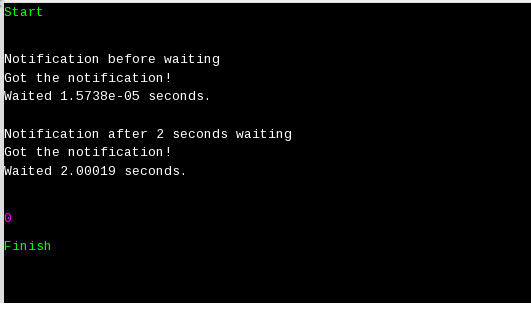
\includegraphics[width=0.4\textwidth]{content/3/chapter6/images/6.png}\\
Thread synchronization
\end{center}

If you compare the class Generator in the infinite data stream with the class Event in this example, there is a subtle difference. In the first case, the Generator is the awaitable and the awaiter; in the second case, the Event uses the operator co\_await to return the awaiter. This separation of concerns into the Awaitable and the awaiter improves the structure of the code.

The output displays that the execution of the second coroutine takes about two seconds. The reason is that the event1 sends its notification (line 119) before the coroutine is suspended, but the event2 sends its notification after a time duration of 2 seconds (line 132).

Now, I put the implementer’s hat on. The workflow of the coroutine is quite challenging to grasp. The class Event has two interesting members: suspendedWaiter and notified. Variable suspendedWaiter in line 31 holds the waiter for the signal, and notified in line 32 has the state of the notification.

In my explanation of both workflows, I assume in the first case (first workflow) that the event notification happens before the coroutine awaits the events. For the second case (second workflow), I assume it is the other way around.

Let’s first look at event1 and the first workflow. Here, event1 sends its notification before receiverThread1 is started. The invocation event1 (line 118) triggers the method notify (lines 75 to 86). First the notification flag is set and then, the call static\_cast<Awaiter*>(suspendedWaiter.load()); loads the potential waiter. In this case, the waiter is a nullptr because it was not set before. This

means the following resume call on the waiter in line 84 is not executed. The subsequentially performed function await\_ready (lines 51 - 61) checks first if there is more than one waiter. In this case, I throw a std::runtime exception. The crucial part of this method is the return value. event.notification was already set to true in the notify method. true means, in this case, that the coroutine is not suspended and executes such as a normal function.

In the second workflow, the co\_await event2 call happens before event2 sends its notification. co\_wait event2 triggers the call await\_ready (line 51). The big difference with the first workflow is that event.notified is false. This false value causes the suspension of the coroutine. Technically, method await\_suspend (lines 63 - 73) is executed. await\_suspend gets the coroutine handle corHandle and stores it for later invocation in the variable coroutineHandle (line 65). Of course, later invocation means resumption. Second, the waiter is stored in the variable suspendedWaiter. When later event2.notify triggers its notification, method notify (line 75) is executed. The difference with the first workflow is that the condition waiter != nullptr evaluates to true. The result is that the waiter uses the coroutineHandle to resume the coroutine.

\begin{tcolorbox}[breakable,enhanced jigsaw,colback=mygreen!5!white,colframe=mygreen!75!black,title={Distilled Information}]
	
\begin{itemize}
\item 
Coroutines are generalized functions that can pause and resume their execution while keeping their state.

\item 
With C++20, we don’t get concrete coroutines, but a framework for implementing coroutines. This framework consists of more than 20 functions that you partially have to implement and partially could overwrite.

\item 
With the new keywords co\_await and co\_yield, C++20 extends the execution of C++ functions with two new concepts.

\item 
Thanks to co\_await expression it is possible to suspend and resume the execution of the expression. If you use co\_await expression in a function func, the call auto getResult = func() does not block if the function’s result is not available. Instead of resource-consuming blocking, you have resource-friendly waiting.

\item 
co\_yield empowers you to write infinite data streams.

\end{itemize}

\end{tcolorbox}



























